\documentclass{article}
\usepackage[utf8]{inputenc}
\usepackage{graphicx}
\usepackage{geometry}
\usepackage{amsmath}
\usepackage{amsfonts}
\usepackage{float}
\usepackage{caption}
\usepackage{subcaption}
\usepackage{enumitem}

\geometry{left=25mm, top=25mm, right=25mm, bottom=25mm}

\title{PHY407 Lab 5}
\author{Pierino Zindel (1002429703) and Hayden Johnson (1002103537)}
\date{October 12, 2018}

\begin{document}

\maketitle

\noindent \textbf{Distribution of work:} Question 1 was completed by Hayden. Question 2 was completed by Pierino.

\section{Basic Applications of the Fourier Transform}

\subsection{a) Newman 7.2: Detecting Periodicity}

\subsubsection{Part a)}

We seek to plot the data contained in the file sunspots.txt and estimate the period of the cyclic component of the data.

A plot of the sunspot data is shown in figure \ref{fig:1a_timeseries}, from which it is clear that there is a regular cycle of fluctuations present in the data. A zoomed in section is shown in figure \ref{fig:1a_timeseries_zoom}, from which it can bee seen that the period of the cycle is roughly:
\begin{align*}
	T &\approx \frac{2970 - 2590}{3} \\
	&\approx 127 \text{months}
\end{align*}

\begin{figure}[H]
	\centering
	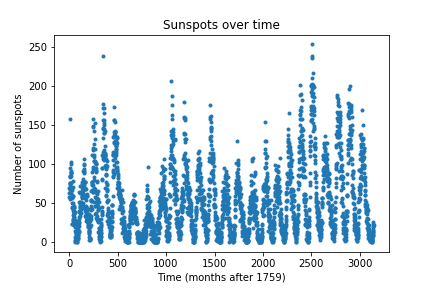
\includegraphics[width=0.8\textwidth]{../images/1a_timeseries.png}
	\caption{Plot showing the number of observed sunspots over time.}
	\label{fig:1a_timeseries}
\end{figure}

\begin{figure}[H]
	\centering
	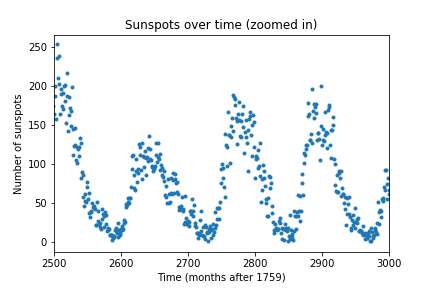
\includegraphics[width=0.8\textwidth]{../images/1a_timeseries_zoomed.png}
	\caption{Zoomed in section of figure \ref{fig:1a_timeseries}.}
	\label{fig:1a_timeseries_zoom}
\end{figure}

\subsubsection{Part b)}

We want to calculate the power spectrum of the sunspot data, and plot it.

The Fourier coefficients of the sunspot data were calculated using np.fft.rfft(), and then the magnitude squared of the coefficients was calculated using np.abs(), which computes the magnitude of a complex number, and squaring this result. A plot of the power spectrum is shown in figure \ref{fig:1a_fourier}. A zoomed in plot of the relevant features is shown in figure \ref{fig:1a_fourier_zoom}, from which it can be seen that there is a clear peak at a non-zero value of $k$.

\begin{figure}[H]
	\centering
	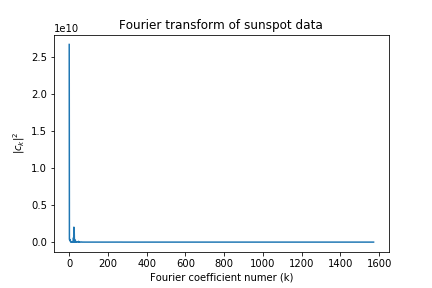
\includegraphics[width=0.8\textwidth]{../images/1a_fourier.png}
	\caption{Fourier transform of the data shown in figure \ref{fig:1a_timeseries}.}
	\label{fig:1a_fourier}
\end{figure}

\begin{figure}[H]
	\centering
	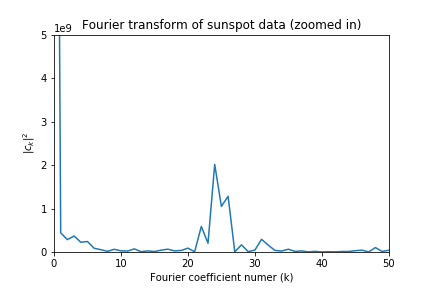
\includegraphics[width=0.8\textwidth]{../images/1a_fourier_zoomed.png}
	\caption{Zoomed in section of figure \ref{fig:1a_fourier}.}
	\label{fig:1a_fourier_zoom}
\end{figure}

\subsubsection{Part c)}

We would like to determine the number of the Fourier coefficient at which the peak occurs, and figure out what period of sine wave corresponds to this number coefficient.

As can be seen from figure \ref{fig:1a_fourier_zoom}, the peak in the Fourier transform occurs at the coefficient with $k\approx 24$. The frequency that corresponds to this number coefficient is:
\begin{equation*}
	f = \frac{k}{L}
\end{equation*}
where $L = 3143$ is the length of the interval covered by the data. Thus, the period is:
\begin{equation*}
	T = \frac{L}{k} = \frac{3143}{24} \approx 131 \text{months}
\end{equation*}
This is in fairly good agreement with the value of $T\approx 127$ months that we found by eye in part a), as we should expect it to be.

\subsection{b) Newman 7.4: Fourier Filtering and Smoothing}

\subsubsection{Part a)}



\section{Newman 7.9: Image Deconvolution}
The Fourier transform is very useful for filtering out noise from a given data set. Extending this principle to a set of two dimensional data that corresponds to an image, we can perform a deconvolution of the image and output a sharper image. This question does exactly this by computing the Fourier transform of a blurry image and a point spread function, combining the two through the relation $a_{kl} = \frac{b_{kl}}{f_{kl}}$ where $a_{kl}$ is the Fourier transform of the clear image data, $b_{kl}$ is the Fourier transform of the blurry image data, and $f_{kl}$ is the Fourier transform of the point spread function.

\subsection{Part a)}
Using the blur.txt data file from Newman's Computational Physics site, a greyscale density plot of the data is shown in figure \ref{fig:blurred_image}. The image appears with high resolution but out of focus which allows us to sharpen the image via this process.

\begin{figure}[H]
	\centering
	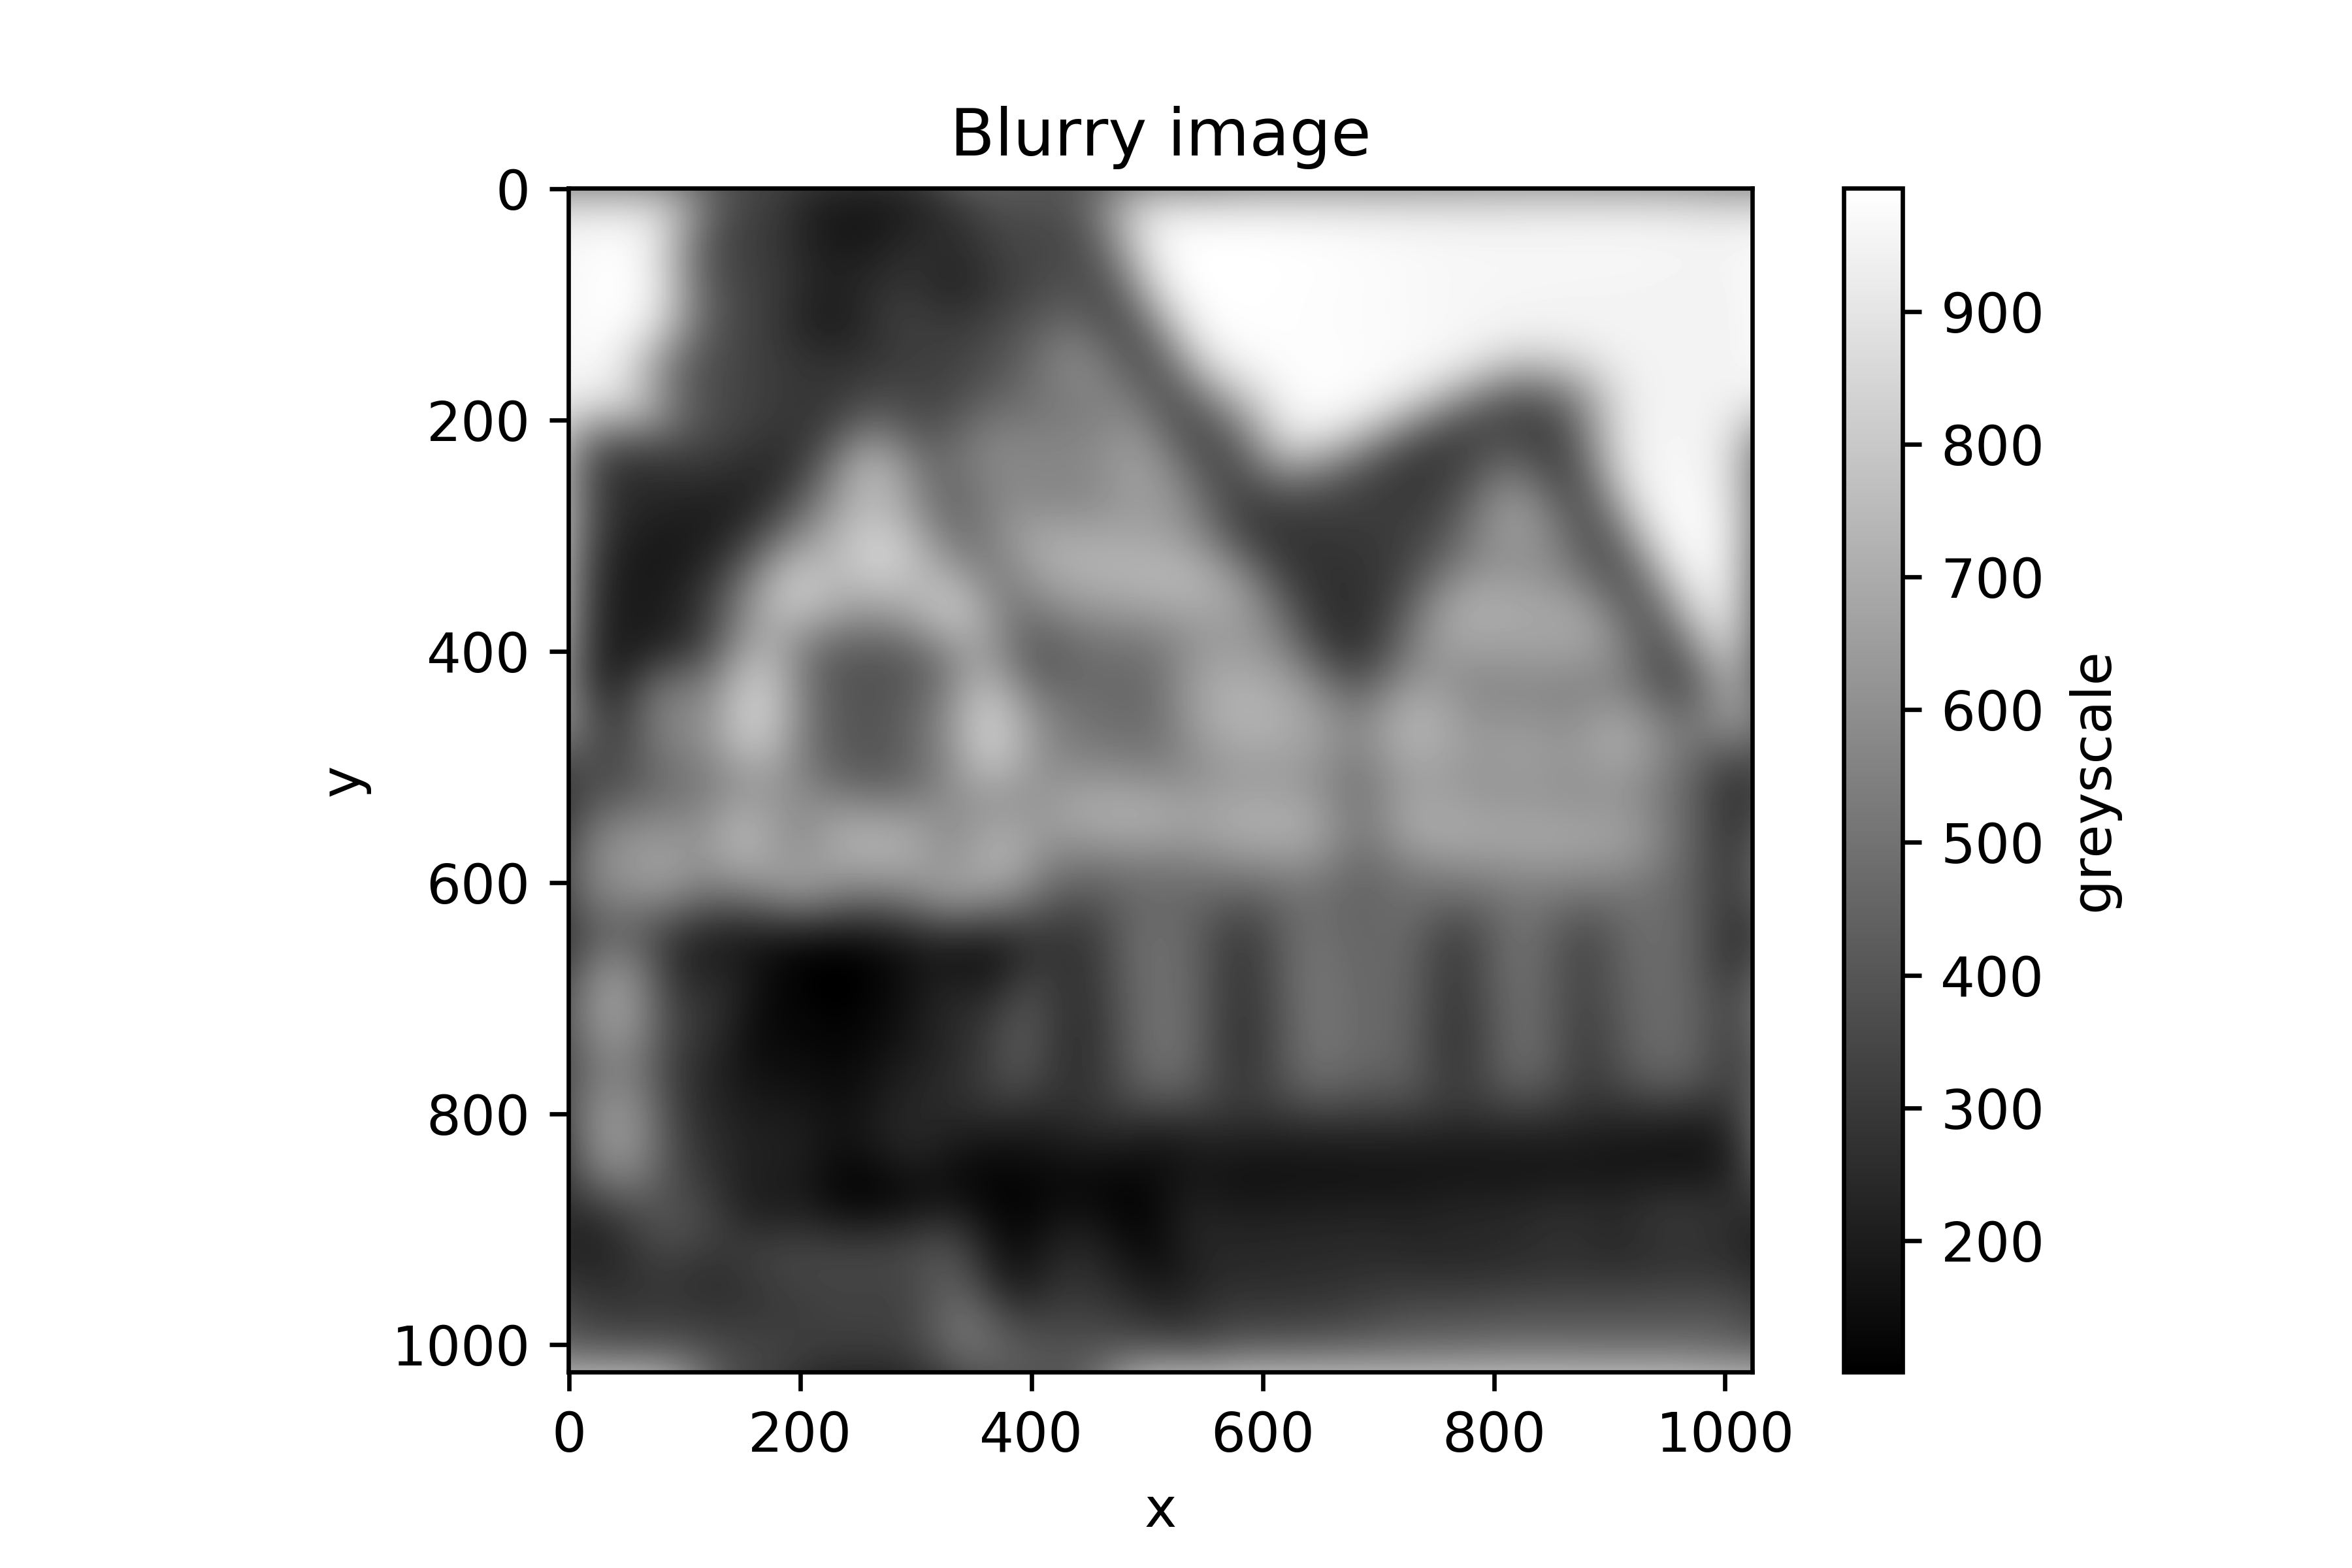
\includegraphics{../images/blurred_image.png}
	\caption{Density plot of provided data shows a blurred image in greyscale.}
	\label{fig:blurred_image}	
\end{figure}

\subsection{Part b)}
The Gaussian point spread function $f(x,y) = exp(-\frac{x^2+y^2}{2\sigma^2}$, periodic in the interval of the original data, was computed for each point of the corresponding blurred image, starting with $(x=0,y=0)$ in the top-left corner. A brightness graph of the spread function is shown in figure \ref{fig:spread_func}

\begin{figure}[H]
	\centering
	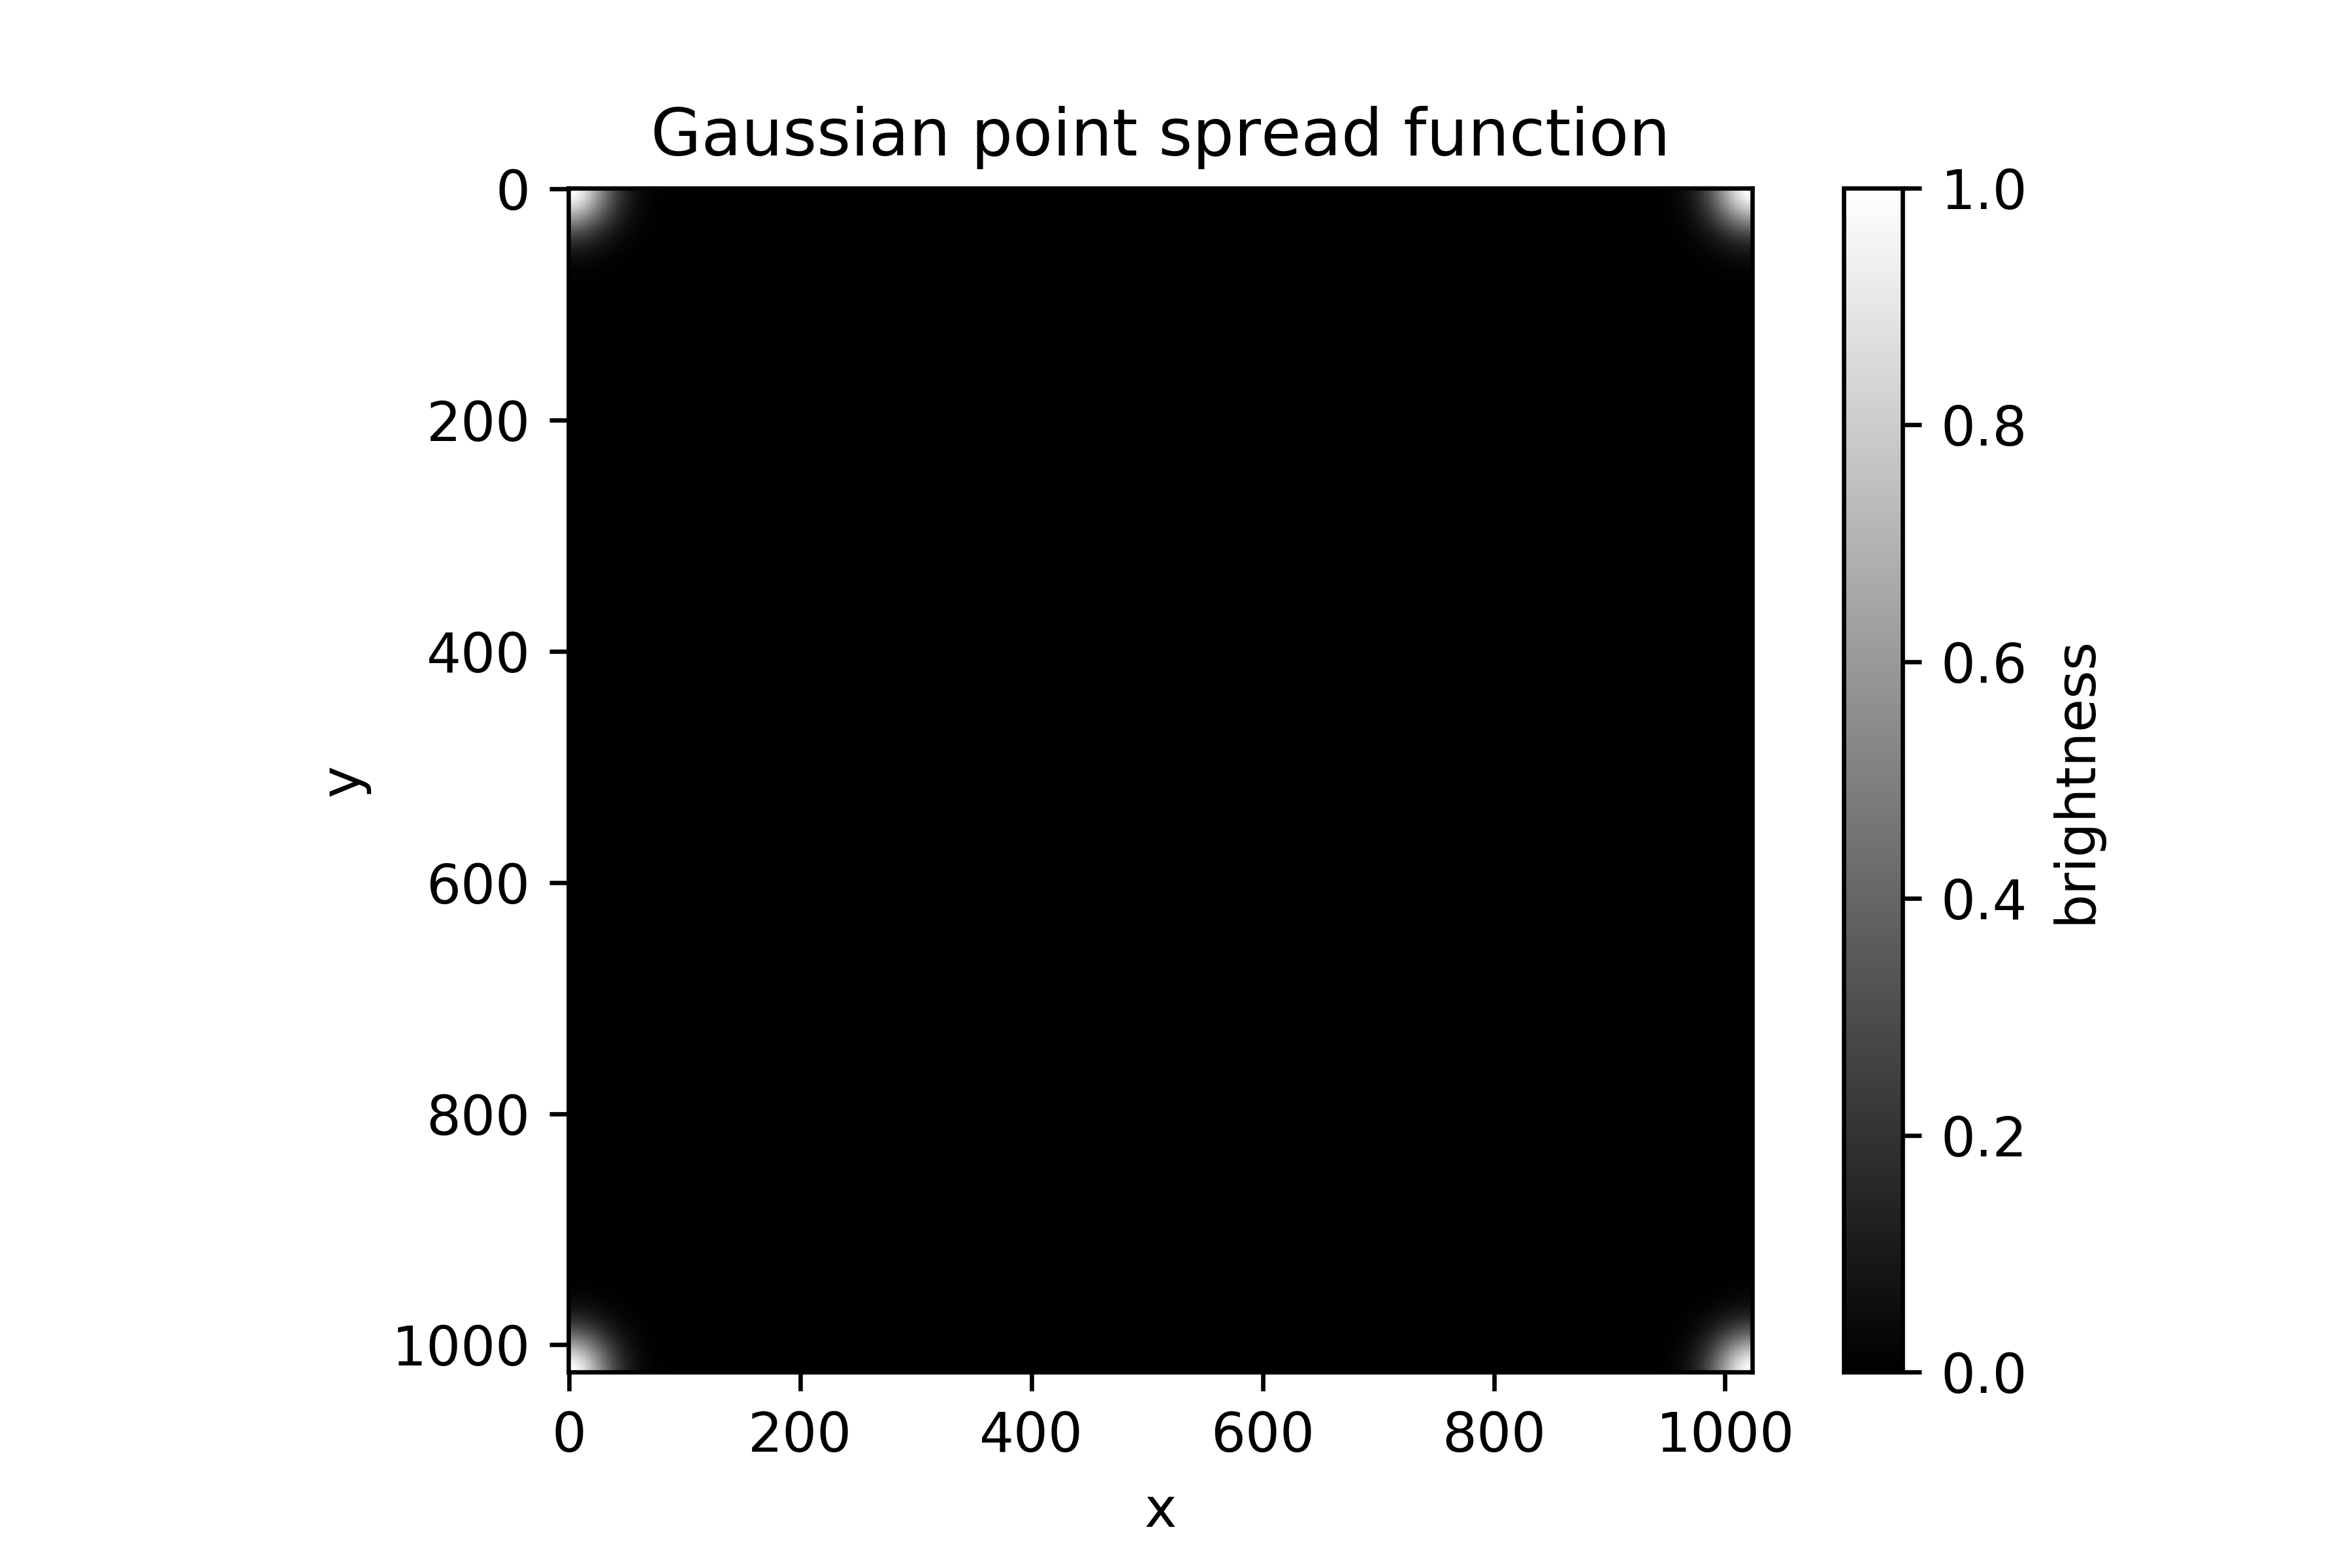
\includegraphics{../images/spread_function.png}
	\caption{Plot of the Gaussian point spread function with $\sigma=25$ used to sharpen the image.}
	\label{fig:spread_func}	
\end{figure}

\subsection{Part c)}
Using the results from part a) and b) we applied a Fourier transform, using the numpy function rfft2, to both the blurred image data set and the spread function data set.
The fft of the blurred image was then divided by the fft of the spread function as described above. To account for the small and possibly zero valued entries in the spread function data set, a cutoff value of $10^{-3}$ was used (wherein the spread function was not applied if the entry values was below the cutoff). Additionally, the textbook notes that the blurred data set should also be divided by the dimensions of the data set, however providing this additional factor resulting in a failure of the deconvolution.
The adjusted fft data was then pass through the inverse, irfft2, function to retrieve a sharpened data set of the original image, which has been graphed in the density plot shown in figure \ref{fig:deconvolved_image}. The resulting image still contains some noise within it however we can now clearly see that the original image was taken of a house with a couple of people walking by in front of it. 

\begin{figure}[H]
	\centering
	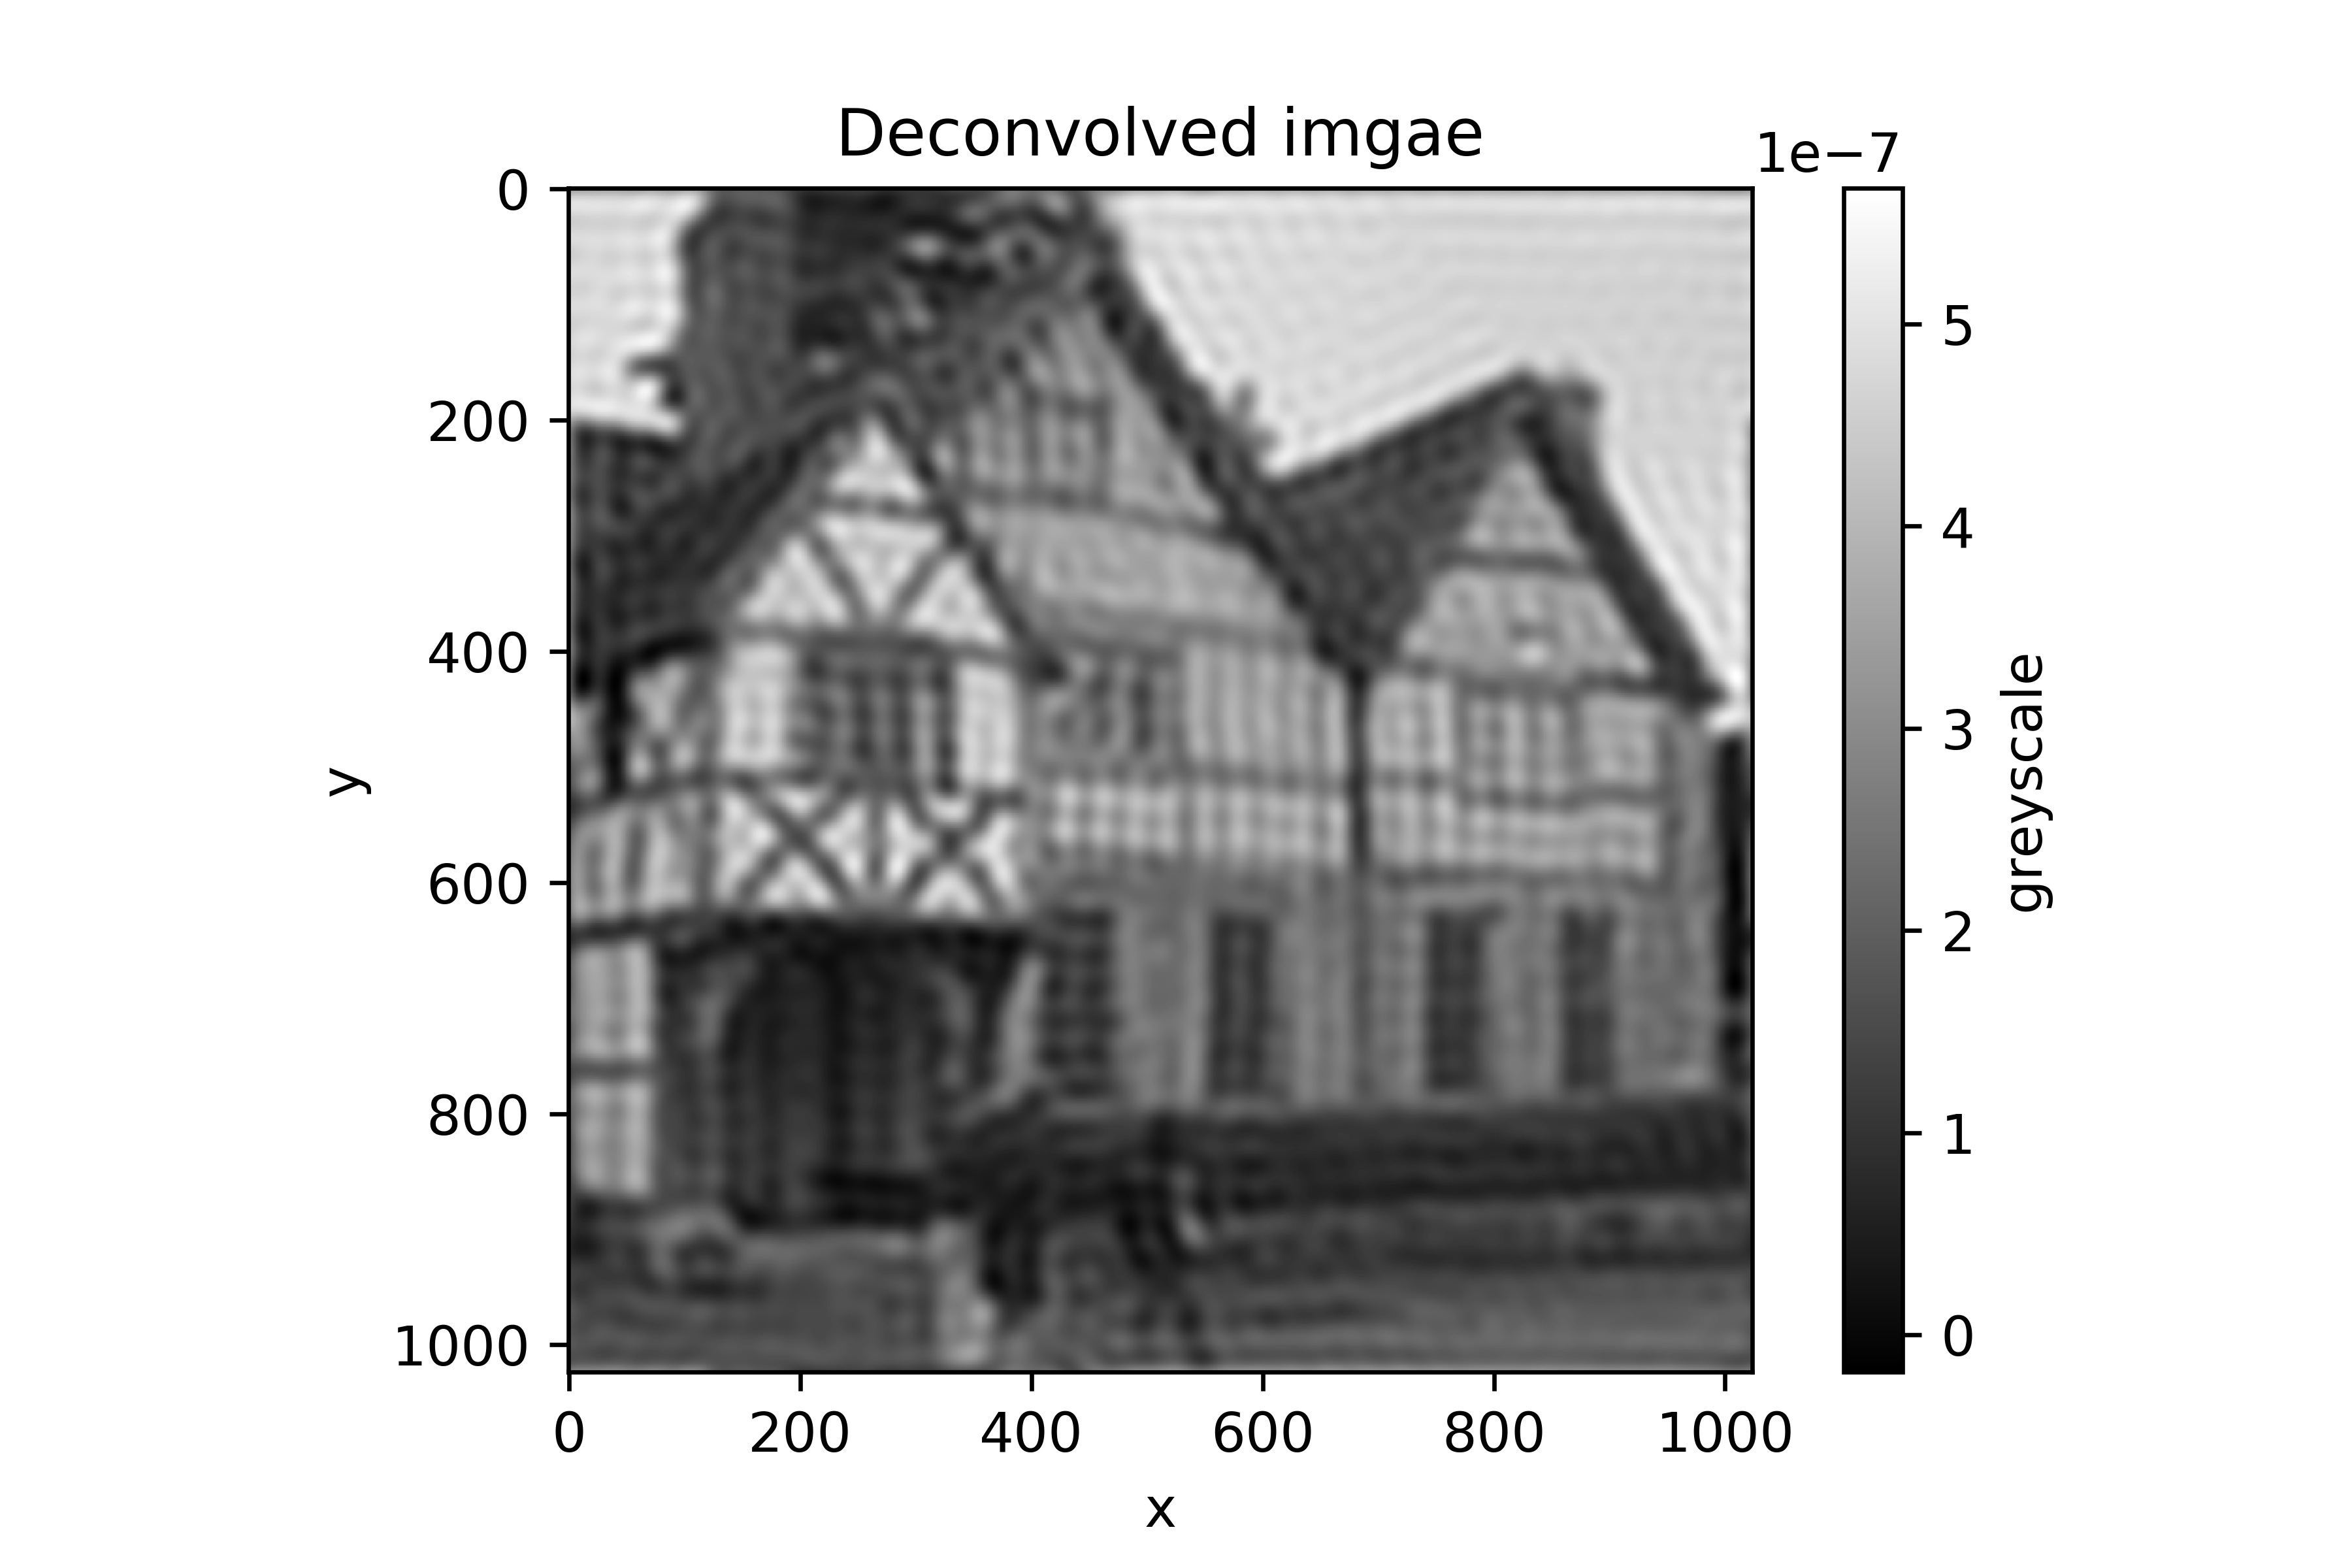
\includegraphics{../images/deconvolved_image.png}
	\caption{Density plot of the greyscale image after applying the spread function via Fourier transform.}
	\label{fig:deconvolved_image}	
\end{figure}

\end{document}